

\tikzset{every picture/.style={line width=0.75pt}} %set default line width to 0.75pt        

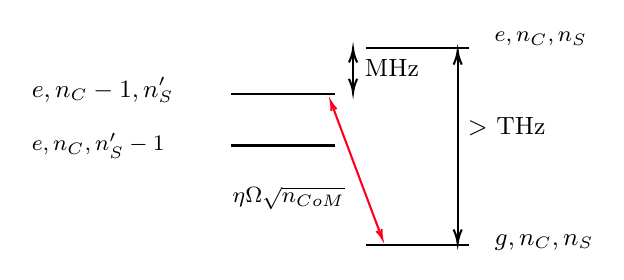
\begin{tikzpicture}[x=0.75pt,y=0.75pt,yscale=-1,xscale=1]
%uncomment if require: \path (0,129); %set diagram left start at 0, and has height of 129

%Straight Lines [id:da1337432598771282] 
\draw    (125.33,63) -- (175.33,63) ;
%Straight Lines [id:da08670055862612258] 
\draw    (125.33,38) -- (175.33,38) ;
%Straight Lines [id:da31987993609756626] 
\draw    (190.33,111) -- (240.33,111) ;
%Straight Lines [id:da6750639847363556] 
\draw    (190.33,16) -- (240.33,16) ;
%Straight Lines [id:da2458293499871056] 
\draw    (184.27,18.42) -- (184.27,35.44) ;
\draw [shift={(184.27,37.44)}, rotate = 270] [color={rgb, 255:red, 0; green, 0; blue, 0 }  ][line width=0.75]    (6.56,-1.97) .. controls (4.17,-0.84) and (1.99,-0.18) .. (0,0) .. controls (1.99,0.18) and (4.17,0.84) .. (6.56,1.97)   ;
\draw [shift={(184.27,16.42)}, rotate = 90] [color={rgb, 255:red, 0; green, 0; blue, 0 }  ][line width=0.75]    (6.56,-1.97) .. controls (4.17,-0.84) and (1.99,-0.18) .. (0,0) .. controls (1.99,0.18) and (4.17,0.84) .. (6.56,1.97)   ;
%Straight Lines [id:da18627337543054923] 
\draw    (234.67,19.44) -- (234.67,108.04) ;
\draw [shift={(234.67,110.04)}, rotate = 270] [color={rgb, 255:red, 0; green, 0; blue, 0 }  ][line width=0.75]    (6.56,-1.97) .. controls (4.17,-0.84) and (1.99,-0.18) .. (0,0) .. controls (1.99,0.18) and (4.17,0.84) .. (6.56,1.97)   ;
\draw [shift={(234.67,17.44)}, rotate = 90] [color={rgb, 255:red, 0; green, 0; blue, 0 }  ][line width=0.75]    (6.56,-1.97) .. controls (4.17,-0.84) and (1.99,-0.18) .. (0,0) .. controls (1.99,0.18) and (4.17,0.84) .. (6.56,1.97)   ;
%Straight Lines [id:da41262627630756243] 
\draw [color={rgb, 255:red, 255; green, 0; blue, 28 }  ,draw opacity=1 ]   (197.62,105.97) -- (174.23,43.71) ;
\draw [shift={(173.53,41.84)}, rotate = 69.41] [color={rgb, 255:red, 255; green, 0; blue, 28 }  ,draw opacity=1 ][line width=0.75]    (4.37,-1.32) .. controls (2.78,-0.56) and (1.32,-0.12) .. (0,0) .. controls (1.32,0.12) and (2.78,0.56) .. (4.37,1.32)   ;
\draw [shift={(198.33,107.84)}, rotate = 249.41] [color={rgb, 255:red, 255; green, 0; blue, 28 }  ,draw opacity=1 ][line width=0.75]    (4.37,-1.32) .. controls (2.78,-0.56) and (1.32,-0.12) .. (0,0) .. controls (1.32,0.12) and (2.78,0.56) .. (4.37,1.32)   ;

% Text Node
\draw (28,28.73) node [anchor=north west][inner sep=0.75pt]  [font=\small]  {$\ket{e,n_{C} -1,n_{S} '}$};
% Text Node
\draw (28,55.73) node [anchor=north west][inner sep=0.75pt]  [font=\footnotesize]  {$\ket{e,n_{C} ,n_{S} '-1}$};
% Text Node
\draw (251,104.4) node [anchor=north west][inner sep=0.75pt]  [font=\small]  {$\ket{g,n_{C} ,n_{S}}$};
% Text Node
\draw (251,6.73) node [anchor=north west][inner sep=0.75pt]  [font=\footnotesize]  {$\ket{e,n_{C} ,n_{S}}$};
% Text Node
\draw (188.51,20.23) node [anchor=north west][inner sep=0.75pt]  [font=\small] [align=left] {{\small MHz}};
% Text Node
\draw (238.11,47.8) node [anchor=north west][inner sep=0.75pt]  [font=\small] [align=left] {{\small $>$ THz}};
% Text Node
\draw (124.8,81.27) node [anchor=north west][inner sep=0.75pt]  [font=\footnotesize]  {$\eta\Omega \sqrt{n_{CoM}}$};


\end{tikzpicture}
